\documentclass[1p]{elsarticle_modified}
%\bibliographystyle{elsarticle-num}

%\usepackage[colorlinks]{hyperref}
%\usepackage{abbrmath_seonhwa} %\Abb, \Ascr, \Acal ,\Abf, \Afrak
\usepackage{amsfonts}
\usepackage{amssymb}
\usepackage{amsmath}
\usepackage{amsthm}
\usepackage{scalefnt}
\usepackage{amsbsy}
\usepackage{kotex}
\usepackage{caption}
\usepackage{subfig}
\usepackage{color}
\usepackage{graphicx}
\usepackage{xcolor} %% white, black, red, green, blue, cyan, magenta, yellow
\usepackage{float}
\usepackage{setspace}
\usepackage{hyperref}

\usepackage{tikz}
\usetikzlibrary{arrows}

\usepackage{multirow}
\usepackage{array} % fixed length table
\usepackage{hhline}

%%%%%%%%%%%%%%%%%%%%%
\makeatletter
\renewcommand*\env@matrix[1][\arraystretch]{%
	\edef\arraystretch{#1}%
	\hskip -\arraycolsep
	\let\@ifnextchar\new@ifnextchar
	\array{*\c@MaxMatrixCols c}}
\makeatother %https://tex.stackexchange.com/questions/14071/how-can-i-increase-the-line-spacing-in-a-matrix
%%%%%%%%%%%%%%%

\usepackage[normalem]{ulem}

\newcommand{\msout}[1]{\ifmmode\text{\sout{\ensuremath{#1}}}\else\sout{#1}\fi}
%SOURCE: \msout is \stkout macro in https://tex.stackexchange.com/questions/20609/strikeout-in-math-mode

\newcommand{\cancel}[1]{
	\ifmmode
	{\color{red}\msout{#1}}
	\else
	{\color{red}\sout{#1}}
	\fi
}

\newcommand{\add}[1]{
	{\color{blue}\uwave{#1}}
}

\newcommand{\replace}[2]{
	\ifmmode
	{\color{red}\msout{#1}}{\color{blue}\uwave{#2}}
	\else
	{\color{red}\sout{#1}}{\color{blue}\uwave{#2}}
	\fi
}

\newcommand{\Sol}{\mathcal{S}} %segment
\newcommand{\D}{D} %diagram
\newcommand{\A}{\mathcal{A}} %arc


%%%%%%%%%%%%%%%%%%%%%%%%%%%%%5 test

\def\sl{\operatorname{\textup{SL}}(2,\Cbb)}
\def\psl{\operatorname{\textup{PSL}}(2,\Cbb)}
\def\quan{\mkern 1mu \triangleright \mkern 1mu}

\theoremstyle{definition}
\newtheorem{thm}{Theorem}[section]
\newtheorem{prop}[thm]{Proposition}
\newtheorem{lem}[thm]{Lemma}
\newtheorem{ques}[thm]{Question}
\newtheorem{cor}[thm]{Corollary}
\newtheorem{defn}[thm]{Definition}
\newtheorem{exam}[thm]{Example}
\newtheorem{rmk}[thm]{Remark}
\newtheorem{alg}[thm]{Algorithm}

\newcommand{\I}{\sqrt{-1}}
\begin{document}

%\begin{frontmatter}
%
%\title{Boundary parabolic representations of knots up to 8 crossings}
%
%%% Group authors per affiliation:
%\author{Yunhi Cho} 
%\address{Department of Mathematics, University of Seoul, Seoul, Korea}
%\ead{yhcho@uos.ac.kr}
%
%
%\author{Seonhwa Kim} %\fnref{s_kim}}
%\address{Center for Geometry and Physics, Institute for Basic Science, Pohang, 37673, Korea}
%\ead{ryeona17@ibs.re.kr}
%
%\author{Hyuk Kim}
%\address{Department of Mathematical Sciences, Seoul National University, Seoul 08826, Korea}
%\ead{hyukkim@snu.ac.kr}
%
%\author{Seokbeom Yoon}
%\address{Department of Mathematical Sciences, Seoul National University, Seoul, 08826,  Korea}
%\ead{sbyoon15@snu.ac.kr}
%
%\begin{abstract}
%We find all boundary parabolic representation of knots up to 8 crossings.
%
%\end{abstract}
%\begin{keyword}
%    \MSC[2010] 57M25 
%\end{keyword}
%
%\end{frontmatter}

%\linenumbers
%\tableofcontents
%
\newcommand\colored[1]{\textcolor{white}{\rule[-0.35ex]{0.8em}{1.4ex}}\kern-0.8em\color{red} #1}%
%\newcommand\colored[1]{\textcolor{white}{ #1}\kern-2.17ex	\textcolor{white}{ #1}\kern-1.81ex	\textcolor{white}{ #1}\kern-2.15ex\color{red}#1	}

{\Large $\underline{11a_{213}~(K11a_{213})}$}

\setlength{\tabcolsep}{10pt}
\renewcommand{\arraystretch}{1.6}
\vspace{1cm}\begin{tabular}{m{100pt}>{\centering\arraybackslash}m{274pt}}
\multirow{5}{120pt}{
	\centering
	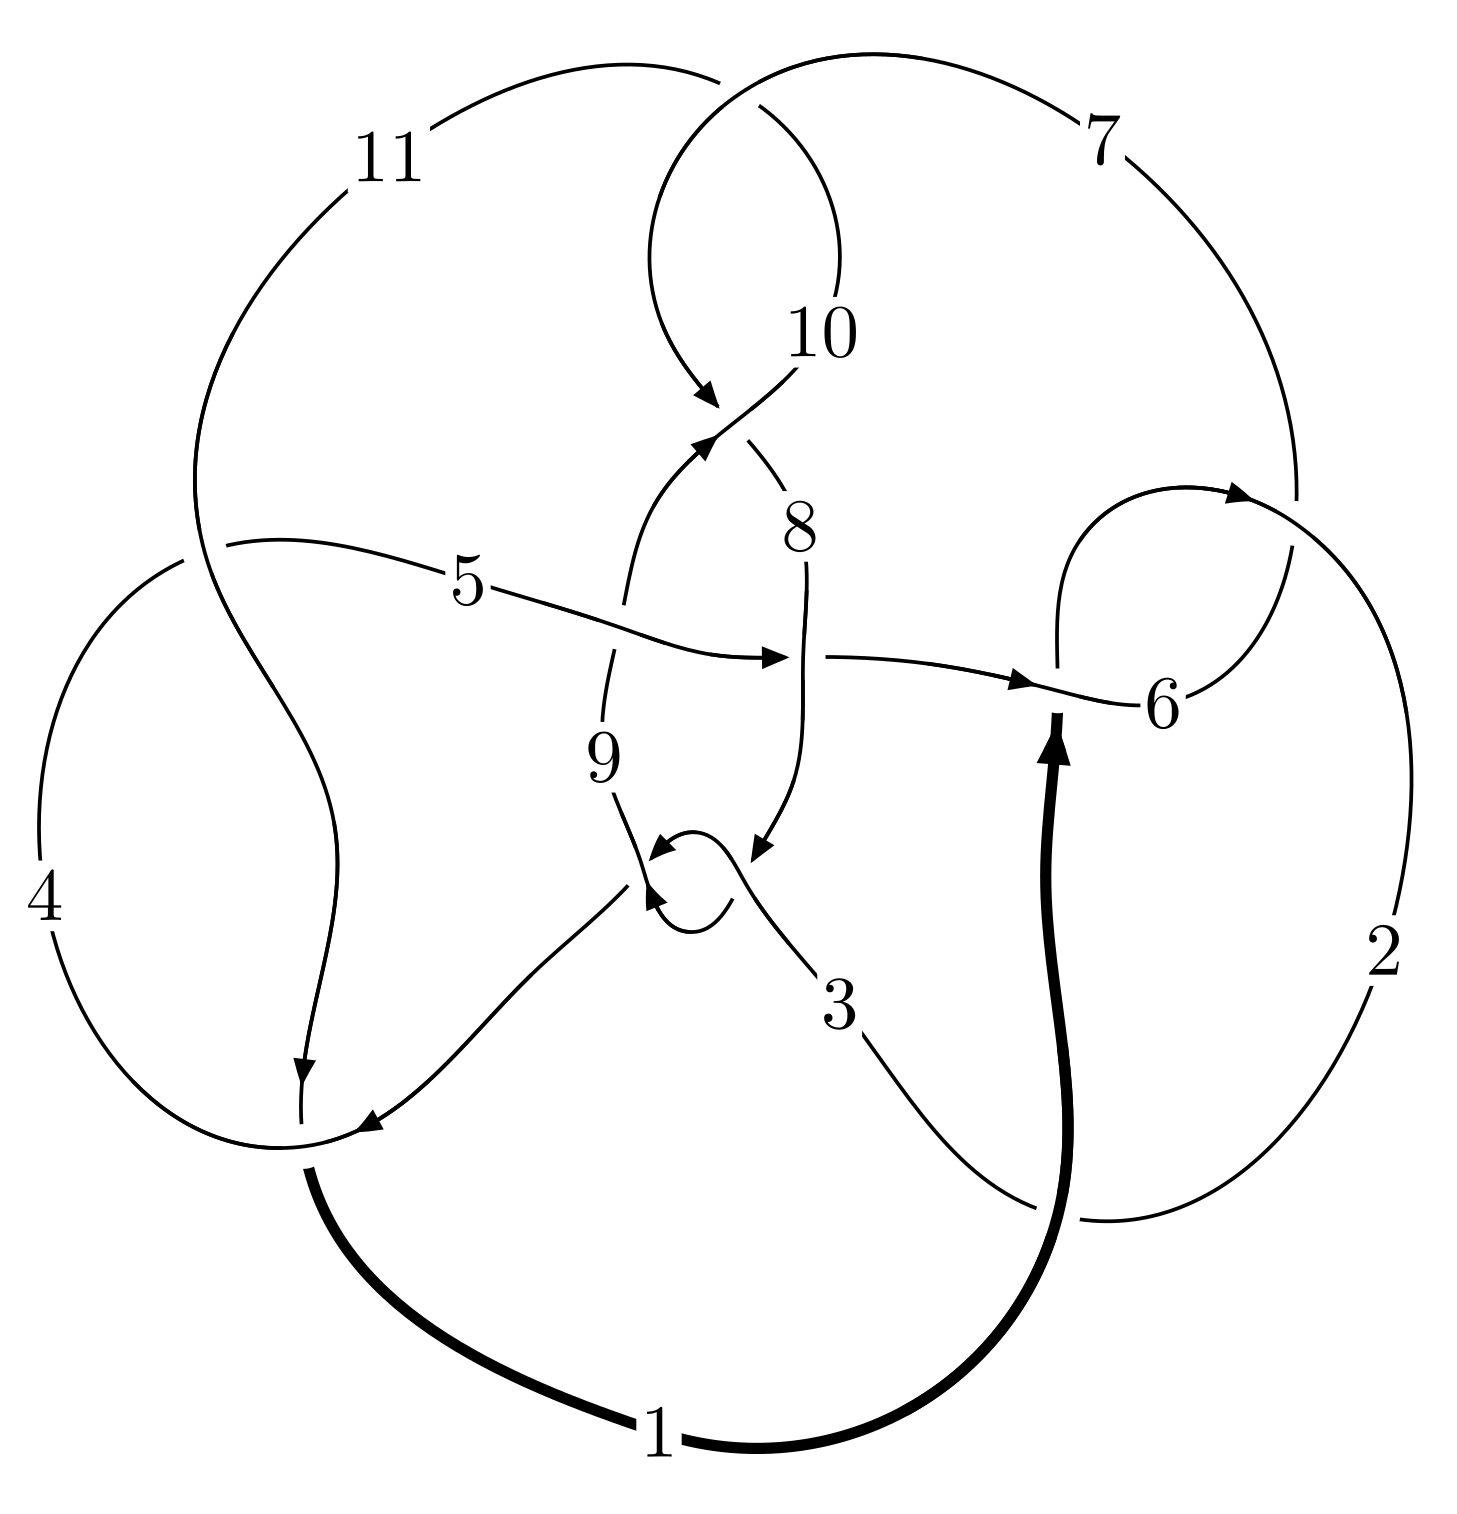
\includegraphics[width=112pt]{../../../GIT/diagram.site/Diagrams/png/462_11a_213.png}\\
\ \ \ A knot diagram\footnotemark}&
\allowdisplaybreaks
\textbf{Linearized knot diagam} \\
\cline{2-2}
 &
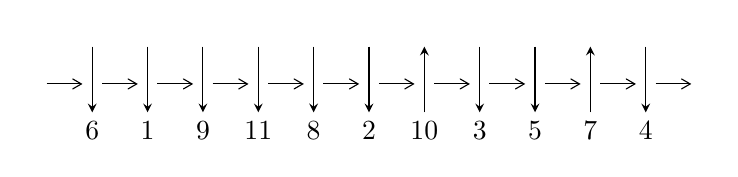
\begin{tikzpicture}[x=20pt, y=17pt]
	% nodes
	\node (C0) at (0, 0) {};
	\node (C1) at (1, 0) {};
	\node (C1U) at (1, +1) {};
	\node (C1D) at (1, -1) {6};

	\node (C2) at (2, 0) {};
	\node (C2U) at (2, +1) {};
	\node (C2D) at (2, -1) {1};

	\node (C3) at (3, 0) {};
	\node (C3U) at (3, +1) {};
	\node (C3D) at (3, -1) {9};

	\node (C4) at (4, 0) {};
	\node (C4U) at (4, +1) {};
	\node (C4D) at (4, -1) {11};

	\node (C5) at (5, 0) {};
	\node (C5U) at (5, +1) {};
	\node (C5D) at (5, -1) {8};

	\node (C6) at (6, 0) {};
	\node (C6U) at (6, +1) {};
	\node (C6D) at (6, -1) {2};

	\node (C7) at (7, 0) {};
	\node (C7U) at (7, +1) {};
	\node (C7D) at (7, -1) {10};

	\node (C8) at (8, 0) {};
	\node (C8U) at (8, +1) {};
	\node (C8D) at (8, -1) {3};

	\node (C9) at (9, 0) {};
	\node (C9U) at (9, +1) {};
	\node (C9D) at (9, -1) {5};

	\node (C10) at (10, 0) {};
	\node (C10U) at (10, +1) {};
	\node (C10D) at (10, -1) {7};

	\node (C11) at (11, 0) {};
	\node (C11U) at (11, +1) {};
	\node (C11D) at (11, -1) {4};
	\node (C12) at (12, 0) {};

	% arrows
	\draw[->,>={angle 60}]
	(C0) edge (C1) (C1) edge (C2) (C2) edge (C3) (C3) edge (C4) (C4) edge (C5) (C5) edge (C6) (C6) edge (C7) (C7) edge (C8) (C8) edge (C9) (C9) edge (C10) (C10) edge (C11) (C11) edge (C12) ;	\draw[->,>=stealth]
	(C1U) edge (C1D) (C2U) edge (C2D) (C3U) edge (C3D) (C4U) edge (C4D) (C5U) edge (C5D) (C6U) edge (C6D) (C7D) edge (C7U) (C8U) edge (C8D) (C9U) edge (C9D) (C10D) edge (C10U) (C11U) edge (C11D) ;
	\end{tikzpicture} \\
\hhline{~~} \\& 
\textbf{Solving Sequence} \\ \cline{2-2} 
 &
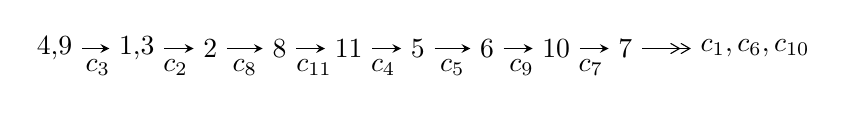
\begin{tikzpicture}[x=25pt, y=7pt]
	% node
	\node (A0) at (-1/8, 0) {4,9};
	\node (A1) at (17/16, 0) {1,3};
	\node (A2) at (17/8, 0) {2};
	\node (A3) at (25/8, 0) {8};
	\node (A4) at (33/8, 0) {11};
	\node (A5) at (41/8, 0) {5};
	\node (A6) at (49/8, 0) {6};
	\node (A7) at (57/8, 0) {10};
	\node (A8) at (65/8, 0) {7};
	\node (C1) at (1/2, -1) {$c_{3}$};
	\node (C2) at (13/8, -1) {$c_{2}$};
	\node (C3) at (21/8, -1) {$c_{8}$};
	\node (C4) at (29/8, -1) {$c_{11}$};
	\node (C5) at (37/8, -1) {$c_{4}$};
	\node (C6) at (45/8, -1) {$c_{5}$};
	\node (C7) at (53/8, -1) {$c_{9}$};
	\node (C8) at (61/8, -1) {$c_{7}$};
	\node (A9) at (10, 0) {$c_{1},c_{6},c_{10}$};

	% edge
	\draw[->,>=stealth]	
	(A0) edge (A1) (A1) edge (A2) (A2) edge (A3) (A3) edge (A4) (A4) edge (A5) (A5) edge (A6) (A6) edge (A7) (A7) edge (A8) ;
	\draw[->>,>={angle 60}]	
	(A8) edge (A9);
\end{tikzpicture} \\ 

\end{tabular} \\

\footnotetext{
The image of knot diagram is generated by the software ``\textbf{Draw programme}" developed by Andrew Bartholomew(\url{http://www.layer8.co.uk/maths/draw/index.htm\#Running-draw}), where we modified some parts for our purpose(\url{https://github.com/CATsTAILs/LinksPainter}).
}\phantom \\ \newline 
\centering \textbf{Ideals for irreducible components\footnotemark of $X_{\text{par}}$} 
 
\begin{align*}
I^u_{1}&=\langle 
-4.59610\times10^{222} u^{91}-6.94766\times10^{222} u^{90}+\cdots+2.72339\times10^{221} b-1.01661\times10^{223},\\
\phantom{I^u_{1}}&\phantom{= \langle  }2.92189\times10^{222} u^{91}+4.36878\times10^{222} u^{90}+\cdots+2.72339\times10^{221} a+5.95579\times10^{222},\;u^{92}+u^{91}+\cdots+u-1\rangle \\
I^u_{2}&=\langle 
21 u^{19}-10 u^{18}+\cdots+b+23,\;5 u^{19}-6 u^{18}+\cdots+a+8,\;u^{20}-6 u^{18}+\cdots+u+1\rangle \\
\\
\end{align*}
\raggedright * 2 irreducible components of $\dim_{\mathbb{C}}=0$, with total 112 representations.\\
\footnotetext{All coefficients of polynomials are rational numbers. But the coefficients are sometimes approximated in decimal forms when there is not enough margin.}
\newpage
\renewcommand{\arraystretch}{1}
\centering \section*{I. $I^u_{1}= \langle -4.60\times10^{222} u^{91}-6.95\times10^{222} u^{90}+\cdots+2.72\times10^{221} b-1.02\times10^{223},\;2.92\times10^{222} u^{91}+4.37\times10^{222} u^{90}+\cdots+2.72\times10^{221} a+5.96\times10^{222},\;u^{92}+u^{91}+\cdots+u-1 \rangle$}
\flushleft \textbf{(i) Arc colorings}\\
\begin{tabular}{m{7pt} m{180pt} m{7pt} m{180pt} }
\flushright $a_{4}=$&$\begin{pmatrix}1\\0\end{pmatrix}$ \\
\flushright $a_{9}=$&$\begin{pmatrix}0\\u\end{pmatrix}$ \\
\flushright $a_{1}=$&$\begin{pmatrix}-10.7288 u^{91}-16.0417 u^{90}+\cdots-20.4887 u-21.8690\\16.8764 u^{91}+25.5110 u^{90}+\cdots+40.6206 u+37.3287\end{pmatrix}$ \\
\flushright $a_{3}=$&$\begin{pmatrix}1\\- u^2\end{pmatrix}$ \\
\flushright $a_{2}=$&$\begin{pmatrix}11.2348 u^{91}+18.9978 u^{90}+\cdots+36.0229 u+34.6600\\-2.18240 u^{91}-2.39881 u^{90}+\cdots-15.0995 u-5.11898\end{pmatrix}$ \\
\flushright $a_{8}=$&$\begin{pmatrix}u\\- u^3+u\end{pmatrix}$ \\
\flushright $a_{11}=$&$\begin{pmatrix}6.14754 u^{91}+9.46936 u^{90}+\cdots+20.1319 u+15.4597\\16.8764 u^{91}+25.5110 u^{90}+\cdots+40.6206 u+37.3287\end{pmatrix}$ \\
\flushright $a_{5}=$&$\begin{pmatrix}-11.4198 u^{91}-18.6265 u^{90}+\cdots-26.8279 u-28.8392\\4.48198 u^{91}+6.96790 u^{90}+\cdots+21.3086 u+14.8116\end{pmatrix}$ \\
\flushright $a_{6}=$&$\begin{pmatrix}-13.4484 u^{91}-22.4378 u^{90}+\cdots-32.7548 u-36.7310\\2.53485 u^{91}+3.73696 u^{90}+\cdots+15.6276 u+8.70253\end{pmatrix}$ \\
\flushright $a_{10}=$&$\begin{pmatrix}5.28893 u^{91}+7.49597 u^{90}+\cdots+10.8597 u+8.11508\\-17.1968 u^{91}-24.5024 u^{90}+\cdots-44.4107 u-35.8919\end{pmatrix}$ \\
\flushright $a_{7}=$&$\begin{pmatrix}-4.97114 u^{91}-5.69526 u^{90}+\cdots-16.4325 u-7.23098\\-14.9240 u^{91}-21.0249 u^{90}+\cdots-36.6876 u-27.4447\end{pmatrix}$\\ \flushright $a_{7}=$&$\begin{pmatrix}-4.97114 u^{91}-5.69526 u^{90}+\cdots-16.4325 u-7.23098\\-14.9240 u^{91}-21.0249 u^{90}+\cdots-36.6876 u-27.4447\end{pmatrix}$\\&\end{tabular}
\flushleft \textbf{(ii) Obstruction class $= -1$}\\~\\
\flushleft \textbf{(iii) Cusp Shapes $= 19.2599 u^{91}+27.9333 u^{90}+\cdots+2.33262 u+18.9254$}\\~\\
\newpage\renewcommand{\arraystretch}{1}
\flushleft \textbf{(iv) u-Polynomials at the component}\newline \\
\begin{tabular}{m{50pt}|m{274pt}}
Crossings & \hspace{64pt}u-Polynomials at each crossing \\
\hline $$\begin{aligned}c_{1},c_{6}\end{aligned}$$&$\begin{aligned}
&u^{92}- u^{91}+\cdots+54 u-143
\end{aligned}$\\
\hline $$\begin{aligned}c_{2}\end{aligned}$$&$\begin{aligned}
&u^{92}+41 u^{91}+\cdots+295208 u+20449
\end{aligned}$\\
\hline $$\begin{aligned}c_{3},c_{8}\end{aligned}$$&$\begin{aligned}
&u^{92}- u^{91}+\cdots- u-1
\end{aligned}$\\
\hline $$\begin{aligned}c_{4},c_{11}\end{aligned}$$&$\begin{aligned}
&u^{92}-3 u^{91}+\cdots+442 u-347
\end{aligned}$\\
\hline $$\begin{aligned}c_{5}\end{aligned}$$&$\begin{aligned}
&u^{92}-3 u^{91}+\cdots+678 u+68
\end{aligned}$\\
\hline $$\begin{aligned}c_{7},c_{10}\end{aligned}$$&$\begin{aligned}
&u^{92}+3 u^{91}+\cdots+734 u+79
\end{aligned}$\\
\hline $$\begin{aligned}c_{9}\end{aligned}$$&$\begin{aligned}
&u^{92}+u^{91}+\cdots-3505 u-387
\end{aligned}$\\
\hline
\end{tabular}\\~\\
\newpage\renewcommand{\arraystretch}{1}
\flushleft \textbf{(v) Riley Polynomials at the component}\newline \\
\begin{tabular}{m{50pt}|m{274pt}}
Crossings & \hspace{64pt}Riley Polynomials at each crossing \\
\hline $$\begin{aligned}c_{1},c_{6}\end{aligned}$$&$\begin{aligned}
&y^{92}-41 y^{91}+\cdots-295208 y+20449
\end{aligned}$\\
\hline $$\begin{aligned}c_{2}\end{aligned}$$&$\begin{aligned}
&y^{92}+31 y^{91}+\cdots-131051768 y+418161601
\end{aligned}$\\
\hline $$\begin{aligned}c_{3},c_{8}\end{aligned}$$&$\begin{aligned}
&y^{92}-51 y^{91}+\cdots-27 y+1
\end{aligned}$\\
\hline $$\begin{aligned}c_{4},c_{11}\end{aligned}$$&$\begin{aligned}
&y^{92}+59 y^{91}+\cdots+3735452 y+120409
\end{aligned}$\\
\hline $$\begin{aligned}c_{5}\end{aligned}$$&$\begin{aligned}
&y^{92}-17 y^{91}+\cdots+950500 y+4624
\end{aligned}$\\
\hline $$\begin{aligned}c_{7},c_{10}\end{aligned}$$&$\begin{aligned}
&y^{92}+49 y^{91}+\cdots-26204 y+6241
\end{aligned}$\\
\hline $$\begin{aligned}c_{9}\end{aligned}$$&$\begin{aligned}
&y^{92}-11 y^{91}+\cdots-5497819 y+149769
\end{aligned}$\\
\hline
\end{tabular}\\~\\
\newpage\flushleft \textbf{(vi) Complex Volumes and Cusp Shapes}
$$\begin{array}{c|c|c}  
\text{Solutions to }I^u_{1}& \I (\text{vol} + \sqrt{-1}CS) & \text{Cusp shape}\\
 \hline 
\begin{aligned}
u &= \phantom{-}0.899956 + 0.428154 I \\
a &= \phantom{-}1.85557 + 0.47759 I \\
b &= \phantom{-}0.010890 - 0.885762 I\end{aligned}
 & \phantom{-}1.37334 + 1.58152 I & \phantom{-0.000000 } 0 \\ \hline\begin{aligned}
u &= \phantom{-}0.899956 - 0.428154 I \\
a &= \phantom{-}1.85557 - 0.47759 I \\
b &= \phantom{-}0.010890 + 0.885762 I\end{aligned}
 & \phantom{-}1.37334 - 1.58152 I & \phantom{-0.000000 } 0 \\ \hline\begin{aligned}
u &= \phantom{-}1.002300 + 0.321909 I \\
a &= \phantom{-}1.082330 - 0.018089 I \\
b &= -0.832463 + 0.052849 I\end{aligned}
 & -0.877139 - 0.912194 I & \phantom{-0.000000 } 0 \\ \hline\begin{aligned}
u &= \phantom{-}1.002300 - 0.321909 I \\
a &= \phantom{-}1.082330 + 0.018089 I \\
b &= -0.832463 - 0.052849 I\end{aligned}
 & -0.877139 + 0.912194 I & \phantom{-0.000000 } 0 \\ \hline\begin{aligned}
u &= -0.802043 + 0.489858 I \\
a &= \phantom{-}1.48741 + 0.08320 I \\
b &= -0.146106 + 1.163070 I\end{aligned}
 & \phantom{-}2.86848 + 1.82626 I & \phantom{-0.000000 } 0 \\ \hline\begin{aligned}
u &= -0.802043 - 0.489858 I \\
a &= \phantom{-}1.48741 - 0.08320 I \\
b &= -0.146106 - 1.163070 I\end{aligned}
 & \phantom{-}2.86848 - 1.82626 I & \phantom{-0.000000 } 0 \\ \hline\begin{aligned}
u &= \phantom{-}0.363192 + 1.037260 I \\
a &= \phantom{-}0.197151 - 0.200110 I \\
b &= \phantom{-}0.385879 - 1.192380 I\end{aligned}
 & \phantom{-}2.46469 + 5.43660 I & \phantom{-0.000000 } 0 \\ \hline\begin{aligned}
u &= \phantom{-}0.363192 - 1.037260 I \\
a &= \phantom{-}0.197151 + 0.200110 I \\
b &= \phantom{-}0.385879 + 1.192380 I\end{aligned}
 & \phantom{-}2.46469 - 5.43660 I & \phantom{-0.000000 } 0 \\ \hline\begin{aligned}
u &= \phantom{-}0.385836 + 0.811407 I \\
a &= \phantom{-}1.25709 - 0.69261 I \\
b &= -0.693377 - 0.983781 I\end{aligned}
 & -2.86301 - 4.52369 I & \phantom{-0.000000 } 0 \\ \hline\begin{aligned}
u &= \phantom{-}0.385836 - 0.811407 I \\
a &= \phantom{-}1.25709 + 0.69261 I \\
b &= -0.693377 + 0.983781 I\end{aligned}
 & -2.86301 + 4.52369 I & \phantom{-0.000000 } 0\\
 \hline 
 \end{array}$$\newpage$$\begin{array}{c|c|c}  
\text{Solutions to }I^u_{1}& \I (\text{vol} + \sqrt{-1}CS) & \text{Cusp shape}\\
 \hline 
\begin{aligned}
u &= -1.093280 + 0.155448 I \\
a &= \phantom{-}0.658445 + 0.311986 I \\
b &= -0.797009 - 0.561932 I\end{aligned}
 & -3.87053 - 2.88480 I & \phantom{-0.000000 } 0 \\ \hline\begin{aligned}
u &= -1.093280 - 0.155448 I \\
a &= \phantom{-}0.658445 - 0.311986 I \\
b &= -0.797009 + 0.561932 I\end{aligned}
 & -3.87053 + 2.88480 I & \phantom{-0.000000 } 0 \\ \hline\begin{aligned}
u &= \phantom{-}1.021630 + 0.504770 I \\
a &= \phantom{-}1.63740 + 0.50649 I \\
b &= -0.86024 - 1.12424 I\end{aligned}
 & \phantom{-}0.75507 - 2.54974 I & \phantom{-0.000000 } 0 \\ \hline\begin{aligned}
u &= \phantom{-}1.021630 - 0.504770 I \\
a &= \phantom{-}1.63740 - 0.50649 I \\
b &= -0.86024 + 1.12424 I\end{aligned}
 & \phantom{-}0.75507 + 2.54974 I & \phantom{-0.000000 } 0 \\ \hline\begin{aligned}
u &= -1.098720 + 0.346642 I \\
a &= \phantom{-}1.299450 + 0.359979 I \\
b &= -1.258100 - 0.118180 I\end{aligned}
 & -4.08734 + 4.93913 I & \phantom{-0.000000 } 0 \\ \hline\begin{aligned}
u &= -1.098720 - 0.346642 I \\
a &= \phantom{-}1.299450 - 0.359979 I \\
b &= -1.258100 + 0.118180 I\end{aligned}
 & -4.08734 - 4.93913 I & \phantom{-0.000000 } 0 \\ \hline\begin{aligned}
u &= \phantom{-}1.020120 + 0.571742 I \\
a &= \phantom{-}0.984851 - 0.334088 I \\
b &= -0.522961 - 0.901176 I\end{aligned}
 & -2.64428 - 2.01886 I & \phantom{-0.000000 } 0 \\ \hline\begin{aligned}
u &= \phantom{-}1.020120 - 0.571742 I \\
a &= \phantom{-}0.984851 + 0.334088 I \\
b &= -0.522961 + 0.901176 I\end{aligned}
 & -2.64428 + 2.01886 I & \phantom{-0.000000 } 0 \\ \hline\begin{aligned}
u &= -1.026570 + 0.575028 I \\
a &= \phantom{-}1.36065 - 0.84820 I \\
b &= -0.50001 + 1.55156 I\end{aligned}
 & \phantom{-}0.762842 + 0.362539 I & \phantom{-0.000000 } 0 \\ \hline\begin{aligned}
u &= -1.026570 - 0.575028 I \\
a &= \phantom{-}1.36065 + 0.84820 I \\
b &= -0.50001 - 1.55156 I\end{aligned}
 & \phantom{-}0.762842 - 0.362539 I & \phantom{-0.000000 } 0\\
 \hline 
 \end{array}$$\newpage$$\begin{array}{c|c|c}  
\text{Solutions to }I^u_{1}& \I (\text{vol} + \sqrt{-1}CS) & \text{Cusp shape}\\
 \hline 
\begin{aligned}
u &= -1.123500 + 0.377477 I \\
a &= -1.82978 + 0.65129 I \\
b &= \phantom{-}0.97324 - 1.09916 I\end{aligned}
 & \phantom{-}0.05662 + 7.54903 I & \phantom{-0.000000 } 0 \\ \hline\begin{aligned}
u &= -1.123500 - 0.377477 I \\
a &= -1.82978 - 0.65129 I \\
b &= \phantom{-}0.97324 + 1.09916 I\end{aligned}
 & \phantom{-}0.05662 - 7.54903 I & \phantom{-0.000000 } 0 \\ \hline\begin{aligned}
u &= \phantom{-}1.138520 + 0.338863 I \\
a &= -1.63737 - 0.79965 I \\
b &= \phantom{-}0.63181 + 1.36847 I\end{aligned}
 & \phantom{-}0.30466 - 3.87854 I & \phantom{-0.000000 } 0 \\ \hline\begin{aligned}
u &= \phantom{-}1.138520 - 0.338863 I \\
a &= -1.63737 + 0.79965 I \\
b &= \phantom{-}0.63181 - 1.36847 I\end{aligned}
 & \phantom{-}0.30466 + 3.87854 I & \phantom{-0.000000 } 0 \\ \hline\begin{aligned}
u &= -0.325891 + 0.743657 I \\
a &= \phantom{-}0.405007 - 0.074605 I \\
b &= -0.791843 - 0.487373 I\end{aligned}
 & -4.17931 - 0.87104 I & -12.11508 + 0. I\phantom{ +0.000000I} \\ \hline\begin{aligned}
u &= -0.325891 - 0.743657 I \\
a &= \phantom{-}0.405007 + 0.074605 I \\
b &= -0.791843 + 0.487373 I\end{aligned}
 & -4.17931 + 0.87104 I & -12.11508 + 0. I\phantom{ +0.000000I} \\ \hline\begin{aligned}
u &= -0.781885 + 0.059041 I \\
a &= -2.52231 - 0.77094 I \\
b &= \phantom{-}1.007020 + 0.764873 I\end{aligned}
 & -2.08061 - 3.09402 I & -11.78916 + 0. I\phantom{ +0.000000I} \\ \hline\begin{aligned}
u &= -0.781885 - 0.059041 I \\
a &= -2.52231 + 0.77094 I \\
b &= \phantom{-}1.007020 - 0.764873 I\end{aligned}
 & -2.08061 + 3.09402 I & -11.78916 + 0. I\phantom{ +0.000000I} \\ \hline\begin{aligned}
u &= -0.687266 + 0.373381 I \\
a &= \phantom{-}1.121870 + 0.778326 I \\
b &= -0.127220 + 1.324110 I\end{aligned}
 & \phantom{-}3.27963 + 2.01059 I & \phantom{-0.000000 } 0. - 2.17901 I \\ \hline\begin{aligned}
u &= -0.687266 - 0.373381 I \\
a &= \phantom{-}1.121870 - 0.778326 I \\
b &= -0.127220 - 1.324110 I\end{aligned}
 & \phantom{-}3.27963 - 2.01059 I & \phantom{-0.000000 -}0. + 2.17901 I\\
 \hline 
 \end{array}$$\newpage$$\begin{array}{c|c|c}  
\text{Solutions to }I^u_{1}& \I (\text{vol} + \sqrt{-1}CS) & \text{Cusp shape}\\
 \hline 
\begin{aligned}
u &= \phantom{-}0.058014 + 1.220800 I \\
a &= \phantom{-}0.276521 + 0.904981 I \\
b &= -0.174273 + 0.678980 I\end{aligned}
 & \phantom{-}1.95041 - 1.39231 I & \phantom{-0.000000 } 0 \\ \hline\begin{aligned}
u &= \phantom{-}0.058014 - 1.220800 I \\
a &= \phantom{-}0.276521 - 0.904981 I \\
b &= -0.174273 - 0.678980 I\end{aligned}
 & \phantom{-}1.95041 + 1.39231 I & \phantom{-0.000000 } 0 \\ \hline\begin{aligned}
u &= \phantom{-}1.174000 + 0.359773 I \\
a &= -1.90983 - 0.96169 I \\
b &= \phantom{-}0.226488 + 1.189200 I\end{aligned}
 & -1.14890 - 7.16658 I & \phantom{-0.000000 } 0 \\ \hline\begin{aligned}
u &= \phantom{-}1.174000 - 0.359773 I \\
a &= -1.90983 + 0.96169 I \\
b &= \phantom{-}0.226488 - 1.189200 I\end{aligned}
 & -1.14890 + 7.16658 I & \phantom{-0.000000 } 0 \\ \hline\begin{aligned}
u &= -1.173860 + 0.371541 I \\
a &= -1.76941 - 0.43236 I \\
b &= \phantom{-}0.536128 - 1.159260 I\end{aligned}
 & -7.03906 + 7.80694 I & \phantom{-0.000000 } 0 \\ \hline\begin{aligned}
u &= -1.173860 - 0.371541 I \\
a &= -1.76941 + 0.43236 I \\
b &= \phantom{-}0.536128 + 1.159260 I\end{aligned}
 & -7.03906 - 7.80694 I & \phantom{-0.000000 } 0 \\ \hline\begin{aligned}
u &= -1.177990 + 0.372709 I \\
a &= -1.37923 + 1.02172 I \\
b &= \phantom{-}0.130525 - 0.776176 I\end{aligned}
 & -0.68335 + 4.74170 I & \phantom{-0.000000 } 0 \\ \hline\begin{aligned}
u &= -1.177990 - 0.372709 I \\
a &= -1.37923 - 1.02172 I \\
b &= \phantom{-}0.130525 + 0.776176 I\end{aligned}
 & -0.68335 - 4.74170 I & \phantom{-0.000000 } 0 \\ \hline\begin{aligned}
u &= \phantom{-}1.154860 + 0.486853 I \\
a &= -1.47799 + 0.52228 I \\
b &= \phantom{-}1.38485 - 0.30163 I\end{aligned}
 & -6.02464 - 10.31350 I & \phantom{-0.000000 } 0 \\ \hline\begin{aligned}
u &= \phantom{-}1.154860 - 0.486853 I \\
a &= -1.47799 - 0.52228 I \\
b &= \phantom{-}1.38485 + 0.30163 I\end{aligned}
 & -6.02464 + 10.31350 I & \phantom{-0.000000 } 0\\
 \hline 
 \end{array}$$\newpage$$\begin{array}{c|c|c}  
\text{Solutions to }I^u_{1}& \I (\text{vol} + \sqrt{-1}CS) & \text{Cusp shape}\\
 \hline 
\begin{aligned}
u &= -0.243416 + 1.236130 I \\
a &= \phantom{-}0.162332 - 0.004245 I \\
b &= -0.489603 - 1.275900 I\end{aligned}
 & \phantom{-}0.85125 - 10.84920 I & \phantom{-0.000000 } 0 \\ \hline\begin{aligned}
u &= -0.243416 - 1.236130 I \\
a &= \phantom{-}0.162332 + 0.004245 I \\
b &= -0.489603 + 1.275900 I\end{aligned}
 & \phantom{-}0.85125 + 10.84920 I & \phantom{-0.000000 } 0 \\ \hline\begin{aligned}
u &= -1.175930 + 0.472649 I \\
a &= -0.633389 - 0.779199 I \\
b &= \phantom{-}0.347606 - 0.779093 I\end{aligned}
 & -6.23055 - 2.15767 I & \phantom{-0.000000 } 0 \\ \hline\begin{aligned}
u &= -1.175930 - 0.472649 I \\
a &= -0.633389 + 0.779199 I \\
b &= \phantom{-}0.347606 + 0.779093 I\end{aligned}
 & -6.23055 + 2.15767 I & \phantom{-0.000000 } 0 \\ \hline\begin{aligned}
u &= \phantom{-}1.214930 + 0.377226 I \\
a &= -1.142750 + 0.184285 I \\
b &= \phantom{-}0.341035 + 1.090410 I\end{aligned}
 & -2.70208 - 3.30839 I & \phantom{-0.000000 } 0 \\ \hline\begin{aligned}
u &= \phantom{-}1.214930 - 0.377226 I \\
a &= -1.142750 - 0.184285 I \\
b &= \phantom{-}0.341035 - 1.090410 I\end{aligned}
 & -2.70208 + 3.30839 I & \phantom{-0.000000 } 0 \\ \hline\begin{aligned}
u &= -1.200470 + 0.459585 I \\
a &= -1.089820 - 0.160696 I \\
b &= \phantom{-}0.851364 + 0.233369 I\end{aligned}
 & -2.24388 + 5.89877 I & \phantom{-0.000000 } 0 \\ \hline\begin{aligned}
u &= -1.200470 - 0.459585 I \\
a &= -1.089820 + 0.160696 I \\
b &= \phantom{-}0.851364 - 0.233369 I\end{aligned}
 & -2.24388 - 5.89877 I & \phantom{-0.000000 } 0 \\ \hline\begin{aligned}
u &= -0.593320 + 1.152030 I \\
a &= \phantom{-}0.247734 + 0.048374 I \\
b &= \phantom{-}0.187453 + 1.138280 I\end{aligned}
 & \phantom{-}4.85118 + 0.81446 I & \phantom{-0.000000 } 0 \\ \hline\begin{aligned}
u &= -0.593320 - 1.152030 I \\
a &= \phantom{-}0.247734 - 0.048374 I \\
b &= \phantom{-}0.187453 - 1.138280 I\end{aligned}
 & \phantom{-}4.85118 - 0.81446 I & \phantom{-0.000000 } 0\\
 \hline 
 \end{array}$$\newpage$$\begin{array}{c|c|c}  
\text{Solutions to }I^u_{1}& \I (\text{vol} + \sqrt{-1}CS) & \text{Cusp shape}\\
 \hline 
\begin{aligned}
u &= \phantom{-}0.695203 + 0.103878 I \\
a &= -2.39103 + 0.60425 I \\
b &= \phantom{-}0.465075 - 0.827446 I\end{aligned}
 & \phantom{-}0.57404 - 1.64965 I & -7.09706 + 2.07909 I \\ \hline\begin{aligned}
u &= \phantom{-}0.695203 - 0.103878 I \\
a &= -2.39103 - 0.60425 I \\
b &= \phantom{-}0.465075 + 0.827446 I\end{aligned}
 & \phantom{-}0.57404 + 1.64965 I & -7.09706 - 2.07909 I \\ \hline\begin{aligned}
u &= \phantom{-}0.656303 + 0.240252 I \\
a &= -0.10956 - 1.42423 I \\
b &= -0.182748 - 1.312790 I\end{aligned}
 & \phantom{-}2.33729 - 4.89796 I & -3.19840 + 10.75719 I \\ \hline\begin{aligned}
u &= \phantom{-}0.656303 - 0.240252 I \\
a &= -0.10956 + 1.42423 I \\
b &= -0.182748 + 1.312790 I\end{aligned}
 & \phantom{-}2.33729 + 4.89796 I & -3.19840 - 10.75719 I \\ \hline\begin{aligned}
u &= -1.30994\phantom{ +0.000000I} \\
a &= -1.00243\phantom{ +0.000000I} \\
b &= \phantom{-}0.647346\phantom{ +0.000000I}\end{aligned}
 & -5.83140\phantom{ +0.000000I} & \phantom{-0.000000 } 0 \\ \hline\begin{aligned}
u &= -1.098340 + 0.736969 I \\
a &= -1.34001 - 0.54457 I \\
b &= \phantom{-}0.653792 - 0.759457 I\end{aligned}
 & -5.90913 + 6.23883 I & \phantom{-0.000000 } 0 \\ \hline\begin{aligned}
u &= -1.098340 - 0.736969 I \\
a &= -1.34001 + 0.54457 I \\
b &= \phantom{-}0.653792 + 0.759457 I\end{aligned}
 & -5.90913 - 6.23883 I & \phantom{-0.000000 } 0 \\ \hline\begin{aligned}
u &= -0.635484 + 0.127279 I \\
a &= -3.48529 - 0.08941 I \\
b &= -0.057611 + 0.532891 I\end{aligned}
 & -3.86440 + 5.70624 I & -8.10788 - 2.00819 I \\ \hline\begin{aligned}
u &= -0.635484 - 0.127279 I \\
a &= -3.48529 + 0.08941 I \\
b &= -0.057611 - 0.532891 I\end{aligned}
 & -3.86440 - 5.70624 I & -8.10788 + 2.00819 I \\ \hline\begin{aligned}
u &= \phantom{-}1.332470 + 0.247847 I \\
a &= -1.007340 + 0.847514 I \\
b &= \phantom{-}0.891796 - 0.453277 I\end{aligned}
 & -9.35815 - 2.58044 I & \phantom{-0.000000 } 0\\
 \hline 
 \end{array}$$\newpage$$\begin{array}{c|c|c}  
\text{Solutions to }I^u_{1}& \I (\text{vol} + \sqrt{-1}CS) & \text{Cusp shape}\\
 \hline 
\begin{aligned}
u &= \phantom{-}1.332470 - 0.247847 I \\
a &= -1.007340 - 0.847514 I \\
b &= \phantom{-}0.891796 + 0.453277 I\end{aligned}
 & -9.35815 + 2.58044 I & \phantom{-0.000000 } 0 \\ \hline\begin{aligned}
u &= \phantom{-}1.239090 + 0.559867 I \\
a &= -0.567349 + 0.606895 I \\
b &= \phantom{-}0.719530 - 0.877837 I\end{aligned}
 & -5.59330 - 0.95533 I & \phantom{-0.000000 } 0 \\ \hline\begin{aligned}
u &= \phantom{-}1.239090 - 0.559867 I \\
a &= -0.567349 - 0.606895 I \\
b &= \phantom{-}0.719530 + 0.877837 I\end{aligned}
 & -5.59330 + 0.95533 I & \phantom{-0.000000 } 0 \\ \hline\begin{aligned}
u &= \phantom{-}1.209370 + 0.632518 I \\
a &= \phantom{-}1.41567 + 0.02861 I \\
b &= -0.62241 - 1.34712 I\end{aligned}
 & -0.21837 - 11.40940 I & \phantom{-0.000000 } 0 \\ \hline\begin{aligned}
u &= \phantom{-}1.209370 - 0.632518 I \\
a &= \phantom{-}1.41567 - 0.02861 I \\
b &= -0.62241 + 1.34712 I\end{aligned}
 & -0.21837 + 11.40940 I & \phantom{-0.000000 } 0 \\ \hline\begin{aligned}
u &= -1.178080 + 0.698481 I \\
a &= \phantom{-}1.180720 - 0.033401 I \\
b &= -0.482051 + 1.253940 I\end{aligned}
 & \phantom{-}2.77259 + 5.73769 I & \phantom{-0.000000 } 0 \\ \hline\begin{aligned}
u &= -1.178080 - 0.698481 I \\
a &= \phantom{-}1.180720 + 0.033401 I \\
b &= -0.482051 - 1.253940 I\end{aligned}
 & \phantom{-}2.77259 - 5.73769 I & \phantom{-0.000000 } 0 \\ \hline\begin{aligned}
u &= -0.359604 + 0.513145 I \\
a &= \phantom{-}1.105950 - 0.461605 I \\
b &= -0.10619 + 1.59127 I\end{aligned}
 & \phantom{-}2.51053 + 4.14874 I & -5.33756 - 6.38441 I \\ \hline\begin{aligned}
u &= -0.359604 - 0.513145 I \\
a &= \phantom{-}1.105950 + 0.461605 I \\
b &= -0.10619 - 1.59127 I\end{aligned}
 & \phantom{-}2.51053 - 4.14874 I & -5.33756 + 6.38441 I \\ \hline\begin{aligned}
u &= \phantom{-}0.188195 + 0.589028 I \\
a &= \phantom{-}1.17085 - 1.73055 I \\
b &= -0.909144 + 0.168813 I\end{aligned}
 & -3.25055 + 5.97769 I & -10.01627 - 5.34702 I\\
 \hline 
 \end{array}$$\newpage$$\begin{array}{c|c|c}  
\text{Solutions to }I^u_{1}& \I (\text{vol} + \sqrt{-1}CS) & \text{Cusp shape}\\
 \hline 
\begin{aligned}
u &= \phantom{-}0.188195 - 0.589028 I \\
a &= \phantom{-}1.17085 + 1.73055 I \\
b &= -0.909144 - 0.168813 I\end{aligned}
 & -3.25055 - 5.97769 I & -10.01627 + 5.34702 I \\ \hline\begin{aligned}
u &= \phantom{-}0.181391 + 0.540978 I \\
a &= \phantom{-}0.789144 - 0.658848 I \\
b &= \phantom{-}0.433458 - 0.123479 I\end{aligned}
 & -0.74698 - 2.02785 I & -4.64089 + 2.72591 I \\ \hline\begin{aligned}
u &= \phantom{-}0.181391 - 0.540978 I \\
a &= \phantom{-}0.789144 + 0.658848 I \\
b &= \phantom{-}0.433458 + 0.123479 I\end{aligned}
 & -0.74698 + 2.02785 I & -4.64089 - 2.72591 I \\ \hline\begin{aligned}
u &= \phantom{-}0.45586 + 1.35944 I \\
a &= \phantom{-}0.146707 + 0.068204 I \\
b &= -0.341442 + 1.074570 I\end{aligned}
 & \phantom{-}3.67608 + 3.90107 I & \phantom{-0.000000 } 0 \\ \hline\begin{aligned}
u &= \phantom{-}0.45586 - 1.35944 I \\
a &= \phantom{-}0.146707 - 0.068204 I \\
b &= -0.341442 - 1.074570 I\end{aligned}
 & \phantom{-}3.67608 - 3.90107 I & \phantom{-0.000000 } 0 \\ \hline\begin{aligned}
u &= -1.32343 + 0.67031 I \\
a &= -1.53002 + 0.19530 I \\
b &= \phantom{-}0.71065 - 1.35618 I\end{aligned}
 & -2.5744 + 17.5099 I & \phantom{-0.000000 } 0 \\ \hline\begin{aligned}
u &= -1.32343 - 0.67031 I \\
a &= -1.53002 - 0.19530 I \\
b &= \phantom{-}0.71065 + 1.35618 I\end{aligned}
 & -2.5744 - 17.5099 I & \phantom{-0.000000 } 0 \\ \hline\begin{aligned}
u &= -0.034570 + 0.494786 I \\
a &= \phantom{-}1.20093 + 1.44391 I \\
b &= -0.111055 - 0.302643 I\end{aligned}
 & \phantom{-}1.16594 - 1.89895 I & -3.75763 + 6.23152 I \\ \hline\begin{aligned}
u &= -0.034570 - 0.494786 I \\
a &= \phantom{-}1.20093 - 1.44391 I \\
b &= -0.111055 + 0.302643 I\end{aligned}
 & \phantom{-}1.16594 + 1.89895 I & -3.75763 - 6.23152 I \\ \hline\begin{aligned}
u &= \phantom{-}1.32427 + 0.73631 I \\
a &= -1.300570 - 0.067697 I \\
b &= \phantom{-}0.573497 + 1.208660 I\end{aligned}
 & \phantom{-}0.67671 - 11.20380 I & \phantom{-0.000000 } 0\\
 \hline 
 \end{array}$$\newpage$$\begin{array}{c|c|c}  
\text{Solutions to }I^u_{1}& \I (\text{vol} + \sqrt{-1}CS) & \text{Cusp shape}\\
 \hline 
\begin{aligned}
u &= \phantom{-}1.32427 - 0.73631 I \\
a &= -1.300570 + 0.067697 I \\
b &= \phantom{-}0.573497 - 1.208660 I\end{aligned}
 & \phantom{-}0.67671 + 11.20380 I & \phantom{-0.000000 } 0 \\ \hline\begin{aligned}
u &= \phantom{-}0.461263 + 0.018499 I \\
a &= -0.73651 - 1.21882 I \\
b &= -0.02599 + 1.55300 I\end{aligned}
 & \phantom{-}2.80824 + 1.36127 I & -5.48968 + 3.29803 I \\ \hline\begin{aligned}
u &= \phantom{-}0.461263 - 0.018499 I \\
a &= -0.73651 + 1.21882 I \\
b &= -0.02599 - 1.55300 I\end{aligned}
 & \phantom{-}2.80824 - 1.36127 I & -5.48968 - 3.29803 I \\ \hline\begin{aligned}
u &= \phantom{-}0.167352 + 0.427245 I \\
a &= \phantom{-}0.761067 + 1.015440 I \\
b &= \phantom{-}0.133945 - 1.282940 I\end{aligned}
 & \phantom{-}2.72282 - 1.44940 I & -5.16116 - 0.05224 I \\ \hline\begin{aligned}
u &= \phantom{-}0.167352 - 0.427245 I \\
a &= \phantom{-}0.761067 - 1.015440 I \\
b &= \phantom{-}0.133945 + 1.282940 I\end{aligned}
 & \phantom{-}2.72282 + 1.44940 I & -5.16116 + 0.05224 I \\ \hline\begin{aligned}
u &= \phantom{-}0.379215\phantom{ +0.000000I} \\
a &= \phantom{-}0.649224\phantom{ +0.000000I} \\
b &= -0.409798\phantom{ +0.000000I}\end{aligned}
 & -0.736675\phantom{ +0.000000I} & -13.9250\phantom{ +0.000000I} \\ \hline\begin{aligned}
u &= -1.62911 + 0.00058 I \\
a &= -0.179116 - 0.487894 I \\
b &= -0.011057 + 0.713112 I\end{aligned}
 & -5.05252 + 1.36520 I & \phantom{-0.000000 } 0 \\ \hline\begin{aligned}
u &= -1.62911 - 0.00058 I \\
a &= -0.179116 + 0.487894 I \\
b &= -0.011057 - 0.713112 I\end{aligned}
 & -5.05252 - 1.36520 I & \phantom{-0.000000 } 0 \\ \hline\begin{aligned}
u &= -0.288297 + 0.213692 I \\
a &= \phantom{-}0.03708 + 1.79806 I \\
b &= -0.45259 - 1.47014 I\end{aligned}
 & \phantom{-}2.55253 - 4.41767 I & -1.66349 + 3.27220 I \\ \hline\begin{aligned}
u &= -0.288297 - 0.213692 I \\
a &= \phantom{-}0.03708 - 1.79806 I \\
b &= -0.45259 + 1.47014 I\end{aligned}
 & \phantom{-}2.55253 + 4.41767 I & -1.66349 - 3.27220 I\\
 \hline 
 \end{array}$$\newpage$$\begin{array}{c|c|c}  
\text{Solutions to }I^u_{1}& \I (\text{vol} + \sqrt{-1}CS) & \text{Cusp shape}\\
 \hline 
\begin{aligned}
u &= \phantom{-}1.67230 + 0.27921 I \\
a &= -0.126637 + 0.712774 I \\
b &= \phantom{-}0.280703 - 0.948609 I\end{aligned}
 & -5.78137 + 4.82781 I & \phantom{-0.000000 } 0 \\ \hline\begin{aligned}
u &= \phantom{-}1.67230 - 0.27921 I \\
a &= -0.126637 - 0.712774 I \\
b &= \phantom{-}0.280703 + 0.948609 I\end{aligned}
 & -5.78137 - 4.82781 I & \phantom{-0.000000 } 0\\
 \hline 
 \end{array}$$\newpage\newpage\renewcommand{\arraystretch}{1}
\centering \section*{II. $I^u_{2}= \langle 21 u^{19}-10 u^{18}+\cdots+b+23,\;5 u^{19}-6 u^{18}+\cdots+a+8,\;u^{20}-6 u^{18}+\cdots+u+1 \rangle$}
\flushleft \textbf{(i) Arc colorings}\\
\begin{tabular}{m{7pt} m{180pt} m{7pt} m{180pt} }
\flushright $a_{4}=$&$\begin{pmatrix}1\\0\end{pmatrix}$ \\
\flushright $a_{9}=$&$\begin{pmatrix}0\\u\end{pmatrix}$ \\
\flushright $a_{1}=$&$\begin{pmatrix}-5 u^{19}+6 u^{18}+\cdots+6 u-8\\-21 u^{19}+10 u^{18}+\cdots+19 u-23\end{pmatrix}$ \\
\flushright $a_{3}=$&$\begin{pmatrix}1\\- u^2\end{pmatrix}$ \\
\flushright $a_{2}=$&$\begin{pmatrix}20 u^{19}-6 u^{18}+\cdots-18 u+21\\-7 u^{19}+5 u^{18}+\cdots+7 u-6\end{pmatrix}$ \\
\flushright $a_{8}=$&$\begin{pmatrix}u\\- u^3+u\end{pmatrix}$ \\
\flushright $a_{11}=$&$\begin{pmatrix}-26 u^{19}+16 u^{18}+\cdots+25 u-31\\-21 u^{19}+10 u^{18}+\cdots+19 u-23\end{pmatrix}$ \\
\flushright $a_{5}=$&$\begin{pmatrix}- u^{18}+5 u^{16}+\cdots-5 u^2+u\\12 u^{19}-10 u^{18}+\cdots-10 u+15\end{pmatrix}$ \\
\flushright $a_{6}=$&$\begin{pmatrix}-5 u^{19}+5 u^{18}+\cdots+3 u-10\\9 u^{19}-7 u^{18}+\cdots-7 u+11\end{pmatrix}$ \\
\flushright $a_{10}=$&$\begin{pmatrix}-4 u^{19}+21 u^{17}+\cdots+5 u^2+4 u\\-21 u^{19}+10 u^{18}+\cdots+15 u-22\end{pmatrix}$ \\
\flushright $a_{7}=$&$\begin{pmatrix}27 u^{19}-21 u^{18}+\cdots-20 u+42\\27 u^{19}-16 u^{18}+\cdots-24 u+34\end{pmatrix}$\\ \flushright $a_{7}=$&$\begin{pmatrix}27 u^{19}-21 u^{18}+\cdots-20 u+42\\27 u^{19}-16 u^{18}+\cdots-24 u+34\end{pmatrix}$\\&\end{tabular}
\flushleft \textbf{(ii) Obstruction class $= 1$}\\~\\
\flushleft \textbf{(iii) Cusp Shapes $= 19 u^{19}-16 u^{18}-101 u^{17}+108 u^{16}+144 u^{15}-213 u^{14}+83 u^{13}-4 u^{12}-327 u^{11}+448 u^{10}+123 u^9-374 u^8+168 u^7-120 u^6-81 u^5+241 u^4+25 u^3-123 u^2-4 u+16$}\\~\\
\newpage\renewcommand{\arraystretch}{1}
\flushleft \textbf{(iv) u-Polynomials at the component}\newline \\
\begin{tabular}{m{50pt}|m{274pt}}
Crossings & \hspace{64pt}u-Polynomials at each crossing \\
\hline $$\begin{aligned}c_{1}\end{aligned}$$&$\begin{aligned}
&u^{20}-5 u^{18}+\cdots-2 u+1
\end{aligned}$\\
\hline $$\begin{aligned}c_{2}\end{aligned}$$&$\begin{aligned}
&u^{20}+10 u^{19}+\cdots+12 u+1
\end{aligned}$\\
\hline $$\begin{aligned}c_{3}\end{aligned}$$&$\begin{aligned}
&u^{20}-6 u^{18}+\cdots+u+1
\end{aligned}$\\
\hline $$\begin{aligned}c_{4}\end{aligned}$$&$\begin{aligned}
&u^{20}+2 u^{19}+\cdots+8 u^2+1
\end{aligned}$\\
\hline $$\begin{aligned}c_{5}\end{aligned}$$&$\begin{aligned}
&u^{20}-4 u^{19}+\cdots-4 u+1
\end{aligned}$\\
\hline $$\begin{aligned}c_{6}\end{aligned}$$&$\begin{aligned}
&u^{20}-5 u^{18}+\cdots+2 u+1
\end{aligned}$\\
\hline $$\begin{aligned}c_{7}\end{aligned}$$&$\begin{aligned}
&u^{20}+4 u^{19}+\cdots+4 u+1
\end{aligned}$\\
\hline $$\begin{aligned}c_{8}\end{aligned}$$&$\begin{aligned}
&u^{20}-6 u^{18}+\cdots- u+1
\end{aligned}$\\
\hline $$\begin{aligned}c_{9}\end{aligned}$$&$\begin{aligned}
&u^{20}+4 u^{17}+\cdots+u+1
\end{aligned}$\\
\hline $$\begin{aligned}c_{10}\end{aligned}$$&$\begin{aligned}
&u^{20}-4 u^{19}+\cdots-4 u+1
\end{aligned}$\\
\hline $$\begin{aligned}c_{11}\end{aligned}$$&$\begin{aligned}
&u^{20}-2 u^{19}+\cdots+8 u^2+1
\end{aligned}$\\
\hline
\end{tabular}\\~\\
\newpage\renewcommand{\arraystretch}{1}
\flushleft \textbf{(v) Riley Polynomials at the component}\newline \\
\begin{tabular}{m{50pt}|m{274pt}}
Crossings & \hspace{64pt}Riley Polynomials at each crossing \\
\hline $$\begin{aligned}c_{1},c_{6}\end{aligned}$$&$\begin{aligned}
&y^{20}-10 y^{19}+\cdots-12 y+1
\end{aligned}$\\
\hline $$\begin{aligned}c_{2}\end{aligned}$$&$\begin{aligned}
&y^{20}+10 y^{19}+\cdots+4 y+1
\end{aligned}$\\
\hline $$\begin{aligned}c_{3},c_{8}\end{aligned}$$&$\begin{aligned}
&y^{20}-12 y^{19}+\cdots-11 y+1
\end{aligned}$\\
\hline $$\begin{aligned}c_{4},c_{11}\end{aligned}$$&$\begin{aligned}
&y^{20}+18 y^{19}+\cdots+16 y+1
\end{aligned}$\\
\hline $$\begin{aligned}c_{5}\end{aligned}$$&$\begin{aligned}
&y^{20}-2 y^{19}+\cdots+8 y+1
\end{aligned}$\\
\hline $$\begin{aligned}c_{7},c_{10}\end{aligned}$$&$\begin{aligned}
&y^{20}+8 y^{19}+\cdots+12 y+1
\end{aligned}$\\
\hline $$\begin{aligned}c_{9}\end{aligned}$$&$\begin{aligned}
&y^{20}-8 y^{17}+\cdots+17 y+1
\end{aligned}$\\
\hline
\end{tabular}\\~\\
\newpage\flushleft \textbf{(vi) Complex Volumes and Cusp Shapes}
$$\begin{array}{c|c|c}  
\text{Solutions to }I^u_{2}& \I (\text{vol} + \sqrt{-1}CS) & \text{Cusp shape}\\
 \hline 
\begin{aligned}
u &= \phantom{-}0.020502 + 1.009610 I \\
a &= \phantom{-}0.239739 - 0.075557 I \\
b &= -0.111980 - 1.179690 I\end{aligned}
 & \phantom{-}4.05337 - 2.46535 I & -3.03812 + 2.80384 I \\ \hline\begin{aligned}
u &= \phantom{-}0.020502 - 1.009610 I \\
a &= \phantom{-}0.239739 + 0.075557 I \\
b &= -0.111980 + 1.179690 I\end{aligned}
 & \phantom{-}4.05337 + 2.46535 I & -3.03812 - 2.80384 I \\ \hline\begin{aligned}
u &= -0.034514 + 1.030530 I \\
a &= \phantom{-}0.417470 - 1.272790 I \\
b &= -0.117330 - 0.725388 I\end{aligned}
 & \phantom{-}2.26277 + 1.45555 I & \phantom{-}6.55534 - 4.54077 I \\ \hline\begin{aligned}
u &= -0.034514 - 1.030530 I \\
a &= \phantom{-}0.417470 + 1.272790 I \\
b &= -0.117330 + 0.725388 I\end{aligned}
 & \phantom{-}2.26277 - 1.45555 I & \phantom{-}6.55534 + 4.54077 I \\ \hline\begin{aligned}
u &= \phantom{-}0.834862 + 0.376425 I \\
a &= -2.85203 + 0.33582 I \\
b &= \phantom{-}0.473306 + 0.639860 I\end{aligned}
 & -4.11080 - 6.47940 I & -11.0697 + 10.5057 I \\ \hline\begin{aligned}
u &= \phantom{-}0.834862 - 0.376425 I \\
a &= -2.85203 - 0.33582 I \\
b &= \phantom{-}0.473306 - 0.639860 I\end{aligned}
 & -4.11080 + 6.47940 I & -11.0697 - 10.5057 I \\ \hline\begin{aligned}
u &= \phantom{-}0.989760 + 0.468800 I \\
a &= \phantom{-}1.42255 + 0.75415 I \\
b &= -0.46915 - 1.35496 I\end{aligned}
 & \phantom{-}1.31973 - 1.14762 I & -5.60070 + 2.26738 I \\ \hline\begin{aligned}
u &= \phantom{-}0.989760 - 0.468800 I \\
a &= \phantom{-}1.42255 - 0.75415 I \\
b &= -0.46915 + 1.35496 I\end{aligned}
 & \phantom{-}1.31973 + 1.14762 I & -5.60070 - 2.26738 I \\ \hline\begin{aligned}
u &= \phantom{-}0.739186 + 0.254368 I \\
a &= \phantom{-}0.812536 + 0.136562 I \\
b &= -0.11506 - 1.54761 I\end{aligned}
 & \phantom{-}2.49233 - 2.11946 I & -10.71875 + 4.52605 I \\ \hline\begin{aligned}
u &= \phantom{-}0.739186 - 0.254368 I \\
a &= \phantom{-}0.812536 - 0.136562 I \\
b &= -0.11506 + 1.54761 I\end{aligned}
 & \phantom{-}2.49233 + 2.11946 I & -10.71875 - 4.52605 I\\
 \hline 
 \end{array}$$\newpage$$\begin{array}{c|c|c}  
\text{Solutions to }I^u_{2}& \I (\text{vol} + \sqrt{-1}CS) & \text{Cusp shape}\\
 \hline 
\begin{aligned}
u &= -1.197310 + 0.297467 I \\
a &= -1.51506 + 1.09231 I \\
b &= \phantom{-}0.456437 - 1.060240 I\end{aligned}
 & -0.69775 + 5.95580 I & -9.18910 - 5.63264 I \\ \hline\begin{aligned}
u &= -1.197310 - 0.297467 I \\
a &= -1.51506 - 1.09231 I \\
b &= \phantom{-}0.456437 + 1.060240 I\end{aligned}
 & -0.69775 - 5.95580 I & -9.18910 + 5.63264 I \\ \hline\begin{aligned}
u &= -0.596304 + 0.330171 I \\
a &= \phantom{-}2.53707 - 0.01833 I \\
b &= -0.918717 + 0.754673 I\end{aligned}
 & -1.49168 + 3.77521 I & -5.50553 - 6.05932 I \\ \hline\begin{aligned}
u &= -0.596304 - 0.330171 I \\
a &= \phantom{-}2.53707 + 0.01833 I \\
b &= -0.918717 - 0.754673 I\end{aligned}
 & -1.49168 - 3.77521 I & -5.50553 + 6.05932 I \\ \hline\begin{aligned}
u &= -0.677664 + 0.019148 I \\
a &= \phantom{-}0.768972 - 0.409121 I \\
b &= -0.36367 - 1.45018 I\end{aligned}
 & \phantom{-}1.86097 - 4.40401 I & -13.93839 + 1.85189 I \\ \hline\begin{aligned}
u &= -0.677664 - 0.019148 I \\
a &= \phantom{-}0.768972 + 0.409121 I \\
b &= -0.36367 + 1.45018 I\end{aligned}
 & \phantom{-}1.86097 + 4.40401 I & -13.93839 - 1.85189 I \\ \hline\begin{aligned}
u &= \phantom{-}1.42090 + 0.17879 I \\
a &= -0.406122 + 0.146508 I \\
b &= -0.189379 + 0.489956 I\end{aligned}
 & -6.67062 + 3.74046 I & -13.8287 - 3.4251 I \\ \hline\begin{aligned}
u &= \phantom{-}1.42090 - 0.17879 I \\
a &= -0.406122 - 0.146508 I \\
b &= -0.189379 - 0.489956 I\end{aligned}
 & -6.67062 - 3.74046 I & -13.8287 + 3.4251 I \\ \hline\begin{aligned}
u &= -1.49942 + 0.05369 I \\
a &= -0.425122 - 0.103178 I \\
b &= \phantom{-}0.355541 + 0.485353 I\end{aligned}
 & -5.59805 - 1.77453 I & -16.1663 + 4.7993 I \\ \hline\begin{aligned}
u &= -1.49942 - 0.05369 I \\
a &= -0.425122 + 0.103178 I \\
b &= \phantom{-}0.355541 - 0.485353 I\end{aligned}
 & -5.59805 + 1.77453 I & -16.1663 - 4.7993 I\\
 \hline 
 \end{array}$$\newpage
\newpage\renewcommand{\arraystretch}{1}
\centering \section*{ III. u-Polynomials}
\begin{tabular}{m{50pt}|m{274pt}}
Crossings & \hspace{64pt}u-Polynomials at each crossing \\
\hline $$\begin{aligned}c_{1}\end{aligned}$$&$\begin{aligned}
&(u^{20}-5 u^{18}+\cdots-2 u+1)(u^{92}- u^{91}+\cdots+54 u-143)
\end{aligned}$\\
\hline $$\begin{aligned}c_{2}\end{aligned}$$&$\begin{aligned}
&(u^{20}+10 u^{19}+\cdots+12 u+1)(u^{92}+41 u^{91}+\cdots+295208 u+20449)
\end{aligned}$\\
\hline $$\begin{aligned}c_{3}\end{aligned}$$&$\begin{aligned}
&(u^{20}-6 u^{18}+\cdots+u+1)(u^{92}- u^{91}+\cdots- u-1)
\end{aligned}$\\
\hline $$\begin{aligned}c_{4}\end{aligned}$$&$\begin{aligned}
&(u^{20}+2 u^{19}+\cdots+8 u^2+1)(u^{92}-3 u^{91}+\cdots+442 u-347)
\end{aligned}$\\
\hline $$\begin{aligned}c_{5}\end{aligned}$$&$\begin{aligned}
&(u^{20}-4 u^{19}+\cdots-4 u+1)(u^{92}-3 u^{91}+\cdots+678 u+68)
\end{aligned}$\\
\hline $$\begin{aligned}c_{6}\end{aligned}$$&$\begin{aligned}
&(u^{20}-5 u^{18}+\cdots+2 u+1)(u^{92}- u^{91}+\cdots+54 u-143)
\end{aligned}$\\
\hline $$\begin{aligned}c_{7}\end{aligned}$$&$\begin{aligned}
&(u^{20}+4 u^{19}+\cdots+4 u+1)(u^{92}+3 u^{91}+\cdots+734 u+79)
\end{aligned}$\\
\hline $$\begin{aligned}c_{8}\end{aligned}$$&$\begin{aligned}
&(u^{20}-6 u^{18}+\cdots- u+1)(u^{92}- u^{91}+\cdots- u-1)
\end{aligned}$\\
\hline $$\begin{aligned}c_{9}\end{aligned}$$&$\begin{aligned}
&(u^{20}+4 u^{17}+\cdots+u+1)(u^{92}+u^{91}+\cdots-3505 u-387)
\end{aligned}$\\
\hline $$\begin{aligned}c_{10}\end{aligned}$$&$\begin{aligned}
&(u^{20}-4 u^{19}+\cdots-4 u+1)(u^{92}+3 u^{91}+\cdots+734 u+79)
\end{aligned}$\\
\hline $$\begin{aligned}c_{11}\end{aligned}$$&$\begin{aligned}
&(u^{20}-2 u^{19}+\cdots+8 u^2+1)(u^{92}-3 u^{91}+\cdots+442 u-347)
\end{aligned}$\\
\hline
\end{tabular}\newpage\renewcommand{\arraystretch}{1}
\centering \section*{ IV. Riley Polynomials}
\begin{tabular}{m{50pt}|m{274pt}}
Crossings & \hspace{64pt}Riley Polynomials at each crossing \\
\hline $$\begin{aligned}c_{1},c_{6}\end{aligned}$$&$\begin{aligned}
&(y^{20}-10 y^{19}+\cdots-12 y+1)(y^{92}-41 y^{91}+\cdots-295208 y+20449)
\end{aligned}$\\
\hline $$\begin{aligned}c_{2}\end{aligned}$$&$\begin{aligned}
&(y^{20}+10 y^{19}+\cdots+4 y+1)\\
&\cdot(y^{92}+31 y^{91}+\cdots-131051768 y+418161601)
\end{aligned}$\\
\hline $$\begin{aligned}c_{3},c_{8}\end{aligned}$$&$\begin{aligned}
&(y^{20}-12 y^{19}+\cdots-11 y+1)(y^{92}-51 y^{91}+\cdots-27 y+1)
\end{aligned}$\\
\hline $$\begin{aligned}c_{4},c_{11}\end{aligned}$$&$\begin{aligned}
&(y^{20}+18 y^{19}+\cdots+16 y+1)\\
&\cdot(y^{92}+59 y^{91}+\cdots+3735452 y+120409)
\end{aligned}$\\
\hline $$\begin{aligned}c_{5}\end{aligned}$$&$\begin{aligned}
&(y^{20}-2 y^{19}+\cdots+8 y+1)(y^{92}-17 y^{91}+\cdots+950500 y+4624)
\end{aligned}$\\
\hline $$\begin{aligned}c_{7},c_{10}\end{aligned}$$&$\begin{aligned}
&(y^{20}+8 y^{19}+\cdots+12 y+1)(y^{92}+49 y^{91}+\cdots-26204 y+6241)
\end{aligned}$\\
\hline $$\begin{aligned}c_{9}\end{aligned}$$&$\begin{aligned}
&(y^{20}-8 y^{17}+\cdots+17 y+1)(y^{92}-11 y^{91}+\cdots-5497819 y+149769)
\end{aligned}$\\
\hline
\end{tabular}
\vskip 2pc
\end{document}